\documentclass[10pt]{article}
\usepackage[T1]{fontenc}
\usepackage{lmodern}
\usepackage[margin=1in]{geometry}
\usepackage{graphicx}
\usepackage{booktabs}
\usepackage{listings}
\usepackage{xcolor}
\usepackage{caption}
\usepackage{float}
\usepackage{microtype}
\usepackage{enumitem}
\usepackage[hidelinks]{hyperref}

\graphicspath{{../}}
\setlist{nosep,leftmargin=1.5em}
\setlength{\parskip}{0.45em}
\setlength{\parindent}{0pt}
\captionsetup{font=small,labelfont=bf}
\lstset{basicstyle=\ttfamily\footnotesize,columns=fullflexible,keepspaces=true,
  frame=single,rulecolor=\color{black!30},xleftmargin=0.5em,xrightmargin=0.5em,
  breaklines=true,aboveskip=0.6em,belowskip=0.6em,float=H}

\newcommand{\code}[1]{\texttt{#1}}

\title{\vspace{-2em}Homework 3: Microarchitecture Reverse Engineering Across Machines}
\author{Manas Reddy Thumma (mrthumm2)\\ECE 492/592, Fall 2026, Track B}
\date{}

\begin{document}
\maketitle
\vspace{-3em}

\section*{Selected questions (115 points)}
\begin{center}
\begin{tabular}{rlr}
\toprule
Q & Exercise & Points\\
\midrule
1 & Confirm the processor is pipelined & 10\\
2 & Confirm out-of-order execution & 10\\
3 & Confirm branch prediction & 10\\
15 & Estimate pipeline depth & 10\\
14 & Estimate instructions fetched per cycle & 10\\
4 & Reverse engineer the ROB size & 30\\
5 & Reverse engineer the physical register file size and class & 35\\
\midrule
 & \textbf{Total} & \textbf{115}\\
\bottomrule
\end{tabular}
\end{center}

\textbf{Machines.} Artemisia (Intel Xeon Gold 5420+, Sapphire Rapids) and Crux (Intel Core i7-9700,
Coffee Lake Refresh).
\textbf{Enclave.} Intel SGX on Artemisia. I did not have SGX access on Crux, where it was off in firmware, so Crux
has native results only.
\textbf{AI use.} Claude Chat helped with the original plan, and Claude Code was used throughout, including running experiments and drafting this report.
See Section~\ref{sec:ai} and \code{AI\_LOG.md}.

\section*{Summary of measured results}
\begin{center}
\small
\begin{tabular}{llll}
\toprule
Q & Crux (native) & Artemisia (native) & Artemisia (SGX)\\
\midrule
1 & Pipelined: add IPC 3.99 vs.\ 1.00 & Pipelined: 4.73 vs.\ 1.00 & Same: 4.72 vs.\ 1.00\\
2 & Out-of-order: 1.02 misses & Out-of-order: 1.04 misses & Same: 1.08 misses\\
3 & Predicts: random 14.4 cycles, & Predicts: random 14.1 cycles, & Same: 14.2 cycles,\\
  & learnable 3.6--5.2 & learnable 2.0--3.6 & learnable 2.0--3.6\\
15 & 19.4 cycles per mispredict & 22.3 cycles & 22.2 cycles\\
14 & 4 instr/cycle, 16 B/cycle & about 6 instr/cycle, $\geq$29 B/cycle & Same\\
4 & ROB $\approx$ 224--225 & ROB $\approx$ 499--500 & Same knee\\
5 & Free int $\approx$ 145, vector $\approx$ 148 & Free int $\approx$ 215, vector $\approx$ 244 & Int 215, vector 263\\
  & Separate classes & Separate classes & Separate classes\\
\bottomrule
\end{tabular}
\end{center}
All conclusions come from timing alone. PMU counters were used only afterwards, as a check.
The main finding across machines: Artemisia's structures are about twice the size of Crux's where the two
differ most (ROB), and the enclave changes memory cost but no core structure.

\section{Machines and setup}
\begin{center}
\small
\begin{tabular}{lll}
\toprule
 & Crux & Artemisia\\
\midrule
CPU & Intel Core i7-9700 @ 3.00 GHz & Intel Xeon Gold 5420+\\
Microarchitecture & Coffee Lake Refresh & Sapphire Rapids (Golden Cove cores)\\
Family / model / stepping & 6 / 158 / 13 & 6 / 143 / 8\\
Topology & 1 socket, 8 cores, no SMT & 2 sockets $\times$ 28 cores $\times$ 2 threads\\
Last-level cache & 12 MiB & 52.5 MiB per socket\\
Kernel & 6.8.0-88 (Ubuntu 24.04.5) & 6.17.8 (el9.elrepo)\\
Compiler / Python & GCC 13.3.0 / 3.12.3 & GCC 11.5.0 / 3.9.25\\
AVX-512 & No & Yes\\
SGX & In the CPU, off in firmware & Yes, used\\
PMU access & Blocked by default (paranoid level 4); & User-space counting available\\
 & set to 2 with sudo for validation only & \\
\bottomrule
\end{tabular}
\end{center}

\textbf{Measurement method.} Every experiment runs through one shared harness, with no machine-specific
code. It pins to one core with \code{taskset} (CPU 2) and reports how busy the SMT sibling is, where one
exists. Times come from \code{rdtsc}. To convert ticks to core cycles, each run times a long dependent
\code{add} chain at 1 add per cycle, and checks the result against a dependent \code{imul} chain, which should
measure 3 cycles. A second calibration at the end of the run records clock drift. Coarse sweeps use 11 trials
and step-1 zooms use 21. Tables report medians, and plots show min--max bands.

\textbf{Enclave platform and configuration.} Intel SGX SDK 2.23, hardware mode, debug enclave, signed with a
self-generated key (possible because the platform has flexible launch control). The kernels, the \code{rdtsc}
reads, the calibration and the test data all run inside the enclave, and the host only handles setup and output. An ECALL
costs about 16k cycles but is never inside a timed region. The heap is static (no EDMM), with 4 KB EPC pages;
native runs also use 4 KB pages so the two are comparable. The LVI mitigation is off because its \code{lfence}s would
serialize the loads these experiments measure, so a production enclave could behave differently.
Native and enclave builds share one driver and the same kernels.

\textbf{Access limitations.} I did not have SGX access on Crux. CPUID reports SGX and launch control, but CPUID leaf 0x12 is empty, with no
\code{sgx} flag and no \code{/dev/sgx*} device. Enabling it needs a firmware change and a reboot of a shared
machine, and the SDK is not installed. I report this as a limitation, and the enclave comparison was done on Artemisia.
PMU counters are not visible inside the enclave, so all PMU checks are native. Crux has no AVX-512, so the
Q5 \code{ymm16--31} test cannot run there.

\section{Q1: Is the processor pipelined?}
\textbf{Method.} Run the same instruction as one dependency chain and as 8 independent chains. A dependent chain
cannot exceed 1/latency instructions per cycle, so an independent version beating that means several instructions
are in flight at once. \code{imul} is the cleanest test: it has 3-cycle latency and a single port, so 1 IPC when
independent means a new multiply enters every cycle while older ones are still in progress.

\begin{lstlisting}
add_dep:   .rept 1000            add_indep: .rept 125
           add %rdx, %rax                   add %rdx, %rax
           .endr                            add %rdx, %rbx   ... 8 registers
                                            .endr
\end{lstlisting}

\begin{figure}[H]\centering
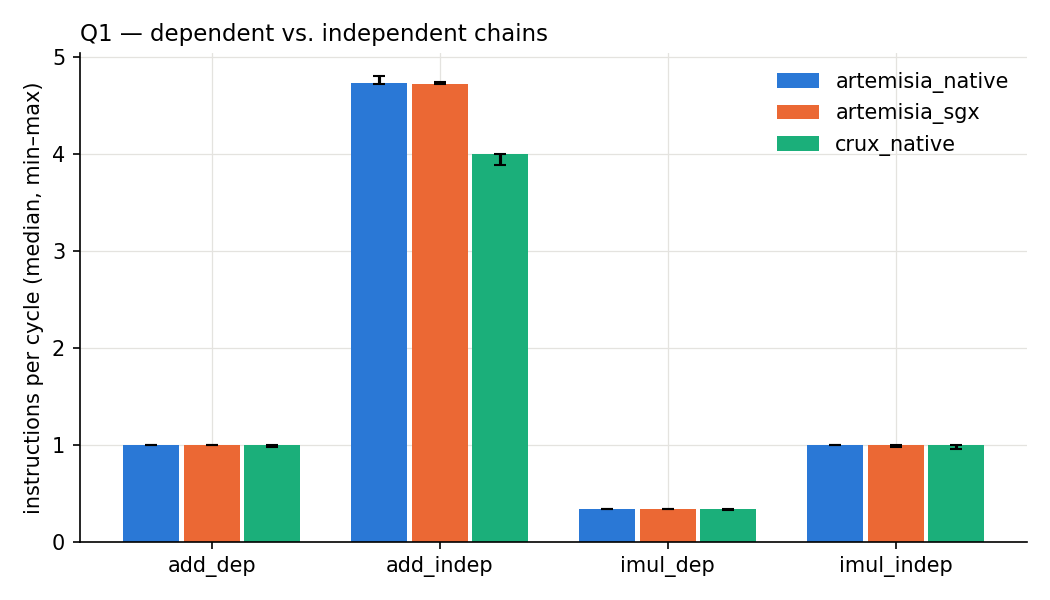
\includegraphics[width=0.62\linewidth]{q01_pipelined/plots/compare/q1_ipc.png}
\caption{Q1: IPC of dependent and independent chains (median, min--max, 11 trials).}
\end{figure}

\begin{center}
\small
\begin{tabular}{lrrrrrr}
\toprule
 & \multicolumn{2}{c}{Crux native} & \multicolumn{2}{c}{Artemisia native} & \multicolumn{2}{c}{Artemisia SGX}\\
Variant & Timing & PMU & Timing & PMU & Timing & PMU\\
\midrule
\code{add\_dep} & 1.000 & 1.001 & 1.000 & 1.001 & 1.001 & --\\
\code{add\_indep} & 3.993 & 4.029 & 4.726 & 4.721 & 4.722 & --\\
\code{imul\_dep} & 0.333 & 0.334 & 0.333 & 0.331 & 0.333 & --\\
\code{imul\_indep} & 1.000 & 1.004 & 1.000 & 1.023 & 1.001 & --\\
\bottomrule
\end{tabular}
\end{center}

\textbf{Conclusion.} Both processors are pipelined and superscalar. On both, independent \code{imul}s run at
three times the rate of dependent ones. Crux's independent \code{add}s reach 3.99 IPC and Artemisia's reach 4.73.
\textbf{Enclave:} no change, as expected for a core property.
\textbf{PMU check:} agrees within 2.3\%. This also validates the cycle calibration, which is otherwise circular
because \code{add\_dep} equals 1 by construction.

\section{Q2: Does the processor execute out of order?}
\textbf{Method.} Two pointer chases run over random cycles of 128 MiB each, far larger than either LLC, so every
load misses to DRAM. Two loads on the same chain must take 2 misses. Two loads on independent chains take about
1 miss if they overlap. Back-to-back overlap alone could also happen on an in-order core with a non-blocking
cache, so the key variant places 4 instructions that consume load A's result before load B. An in-order core
would stall at those consumers, and only an out-of-order core can issue B past them.

\begin{lstlisting}
1:  mov (%rax), %rax    # load A (chain p): misses
    lea 1(%rax), %r8    # consumers of A: an in-order core stalls here
    add %r8, %r9
    add %r9, %r10
    add %r10, %r11
    mov (%rcx), %rcx    # load B (chain q): independent miss
    dec %rdx
    jnz 1b
\end{lstlisting}

\begin{figure}[H]\centering
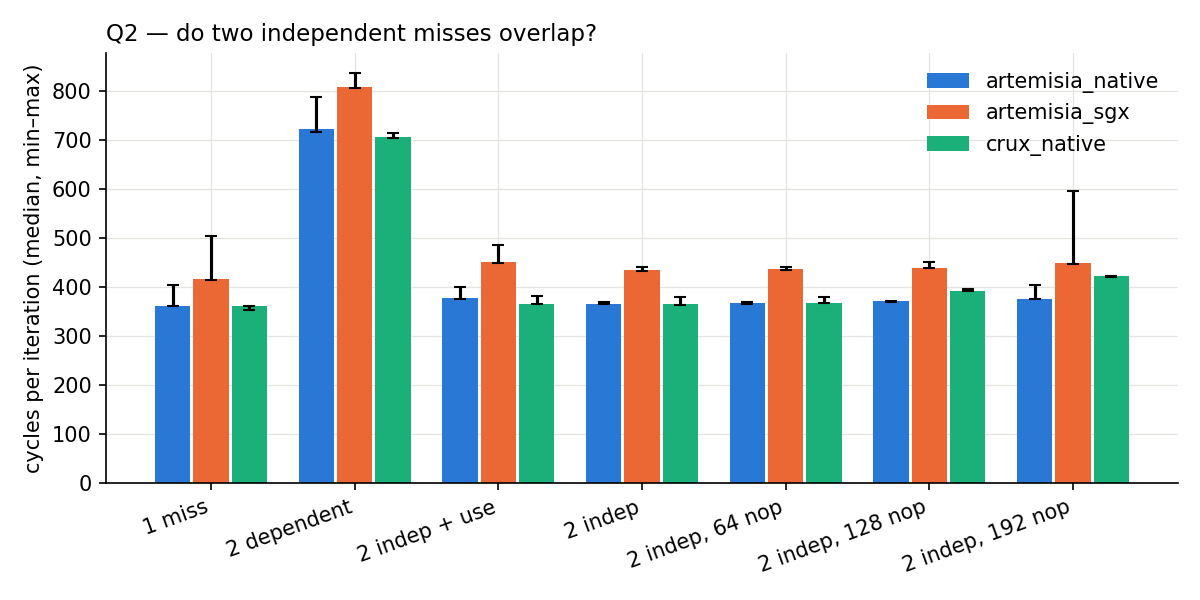
\includegraphics[width=0.72\linewidth]{q02_ooo/plots/compare/q2_overlap.png}
\caption{Q2: cycles per iteration by variant (median, min--max, 11 trials).}
\end{figure}

\begin{center}
\small
\begin{tabular}{lrrrrrr}
\toprule
 & \multicolumn{2}{c}{Crux native} & \multicolumn{2}{c}{Artemisia native} & \multicolumn{2}{c}{Artemisia SGX}\\
Variant & Cycles & Misses & Cycles & Misses & Cycles & Misses\\
\midrule
1 miss & 360 & 1.00 & 361 & 1.00 & 415 & 1.00\\
2 dependent & 705 & 1.96 & 722 & 2.00 & 808 & 1.94\\
2 independent, with consumers & 366 & 1.02 & 377 & 1.04 & 451 & 1.08\\
2 independent & 365 & 1.01 & 366 & 1.01 & 434 & 1.04\\
2 independent, 64 NOPs & 368 & 1.02 & 367 & 1.02 & 436 & 1.05\\
2 independent, 128 NOPs & 392 & 1.09 & 370 & 1.03 & 440 & 1.06\\
2 independent, 192 NOPs & 422 & 1.17 & 376 & 1.04 & 448 & 1.08\\
\bottomrule
\end{tabular}
\end{center}

\textbf{Conclusion.} Both processors execute out of order: with consumers in between, two misses still cost about one.
\textbf{Machine difference:} 192 NOPs cost Crux more (1.17 misses vs.\ 1.04), which fits a narrower core taking
longer to get through the filler and a ROB of 224 sitting close to that filler size.
\textbf{Enclave:} a miss costs 15\% more (415 vs.\ 361 cycles), consistent with encrypted EPC memory, and the conclusion is the same.
\textbf{PMU check:} not performed.

\section{Q3: Does the processor predict branches?}
\textbf{Method.} A loop executes one conditional branch per array element, driven by the element's value. Both
paths do one \code{add}, so patterns differ only in predictability. If a random 50/50 pattern costs far more than
learnable patterns with the same direction mix, the processor is speculating on direction. The branch is in
assembly so the compiler cannot turn it into a \code{cmov}. Each pattern array is 1 MiB, trained with one pass, then timed over 4 passes.

\begin{lstlisting}
.Lloop:  movzbl (%rdi,%rcx), %r8d
         test   %r8d, %r8d
         jnz    .Ltaken          # <-- branch under test
         add    %r10, %r9
         jmp    .Ljoin
.Ltaken: add    %r10, %rax
.Ljoin:  inc    %rcx
         cmp    %rsi, %rcx
         jb     .Lloop
\end{lstlisting}

\begin{figure}[H]\centering
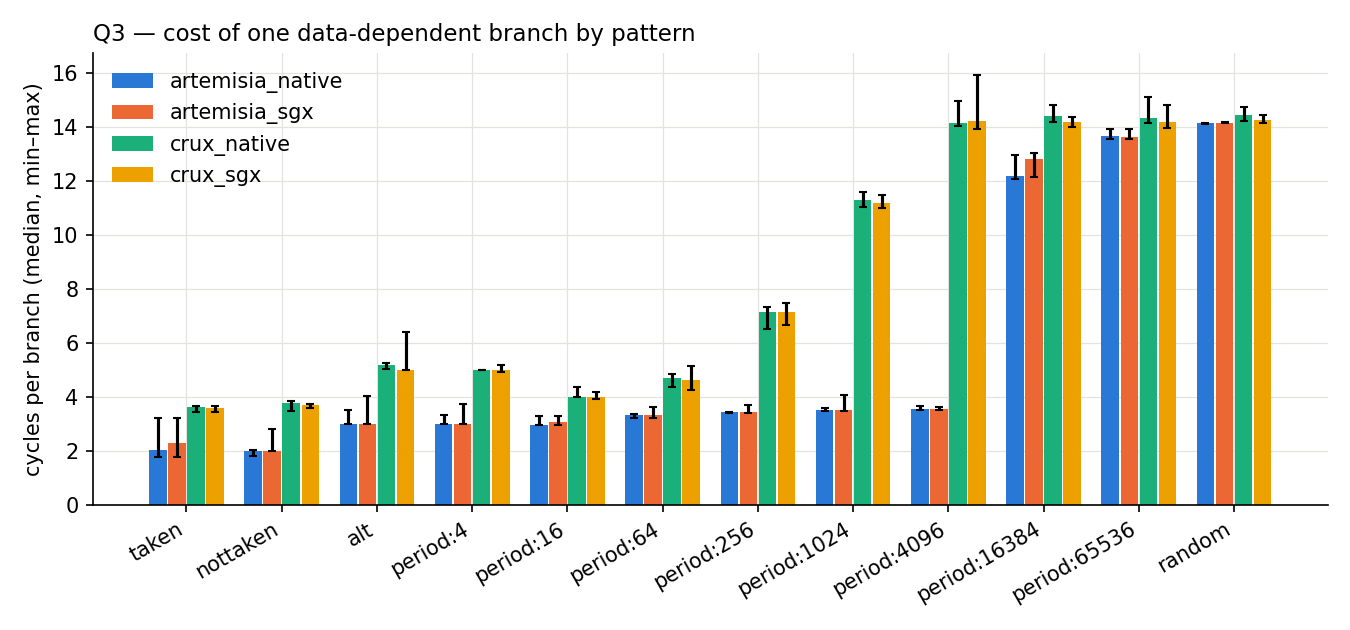
\includegraphics[width=0.85\linewidth]{q03_branch/plots/compare/q3_branch.png}
\caption{Q3: cycles per branch by pattern (median, min--max, 11 trials).}
\end{figure}

\begin{center}
\small
\begin{tabular}{lrrrrrr}
\toprule
 & \multicolumn{3}{c}{Crux native} & \multicolumn{3}{c}{Artemisia} \\
Pattern & Timing & PMU & Miss rate & Timing & PMU & SGX timing\\
\midrule
\code{taken} & 3.60 & 3.51 & 0.00000 & 2.01 & 1.85 & 2.30\\
\code{nottaken} & 3.77 & 4.04 & 0.00000 & 2.00 & 2.05 & 2.00\\
\code{alt} & 5.16 & 4.99 & 0.00001 & 3.00 & 2.66 & 3.00\\
\code{period:16} & 4.01 & 4.33 & 0.00000 & 2.95 & 3.03 & 3.07\\
\code{period:64} & 4.71 & -- & -- & 3.33 & -- & 3.33\\
\code{period:256} & 7.13 & -- & -- & 3.42 & -- & 3.43\\
\code{period:1024} & 11.30 & -- & -- & 3.50 & -- & 3.49\\
\code{period:4096} & 14.16 & -- & -- & 3.55 & -- & 3.55\\
\code{period:16384} & 14.41 & -- & -- & 12.18 & -- & 12.83\\
\code{period:65536} & 14.35 & -- & -- & 13.68 & -- & 13.62\\
\code{random} & 14.43 & 14.24 & 0.49994 & 14.14 & 14.28 & 14.16\\
\bottomrule
\end{tabular}
\end{center}

\textbf{Conclusion.} Both processors predict branches. Random costs about 9--11 cycles more per branch than
learnable patterns with the same mix.
\textbf{Machine difference:} Artemisia learns patterns up to period 4096, while Crux starts degrading by period 256 and reaches
random-level cost at period 4096. This is consistent with a smaller history or table capacity on Crux, though I did not isolate which.
\textbf{Enclave:} identical within noise.
\textbf{PMU check:} the slow pattern misses at 0.5 and the fast ones at essentially 0, on both machines (Artemisia's
\code{random} miss rate is 0.49967).
\textbf{Open question:} on Crux, no-miss patterns still cost 3.5--5.0 cycles, with \code{alt} the most expensive.
PMU shows this is not misprediction, so the cause is probably in the front end. I did not measure the cause.
The JCC erratum microcode mitigation is one candidate, but this is untested.

\section{Q15: How deep is the pipeline?}
\textbf{Method (timing only).} A mispredict discards fetched work, and the front end must refill. Time lost per mispredict therefore
estimates the distance from the front end to branch resolution. It is a \emph{lower bound} on depth, not a stage count, because it
excludes stages after execute and overlap can hide part of it. The difficulty without counters is knowing the number of mispredicts. A
fair coin solves this: for independent 50/50 outcomes, every predictor misses half the time in expectation, because nothing it can observe
helps. With a perfectly predicted pattern as the baseline:

\begin{lstlisting}
P   = (t["bias:0.50"] - t["alt"]) / 0.5          # same 50/50 path mix, no mispredicts
P16 = (t["bias:0.50"] - t["period:16"]) / 0.5    # alternative baseline, shows sensitivity
\end{lstlisting}

Dividing by min($F$, $1-F$) at other taken probabilities $F$ gives only an upper bound on $P$, since real predictors miss more than that on biased noise.

\begin{figure}[H]\centering
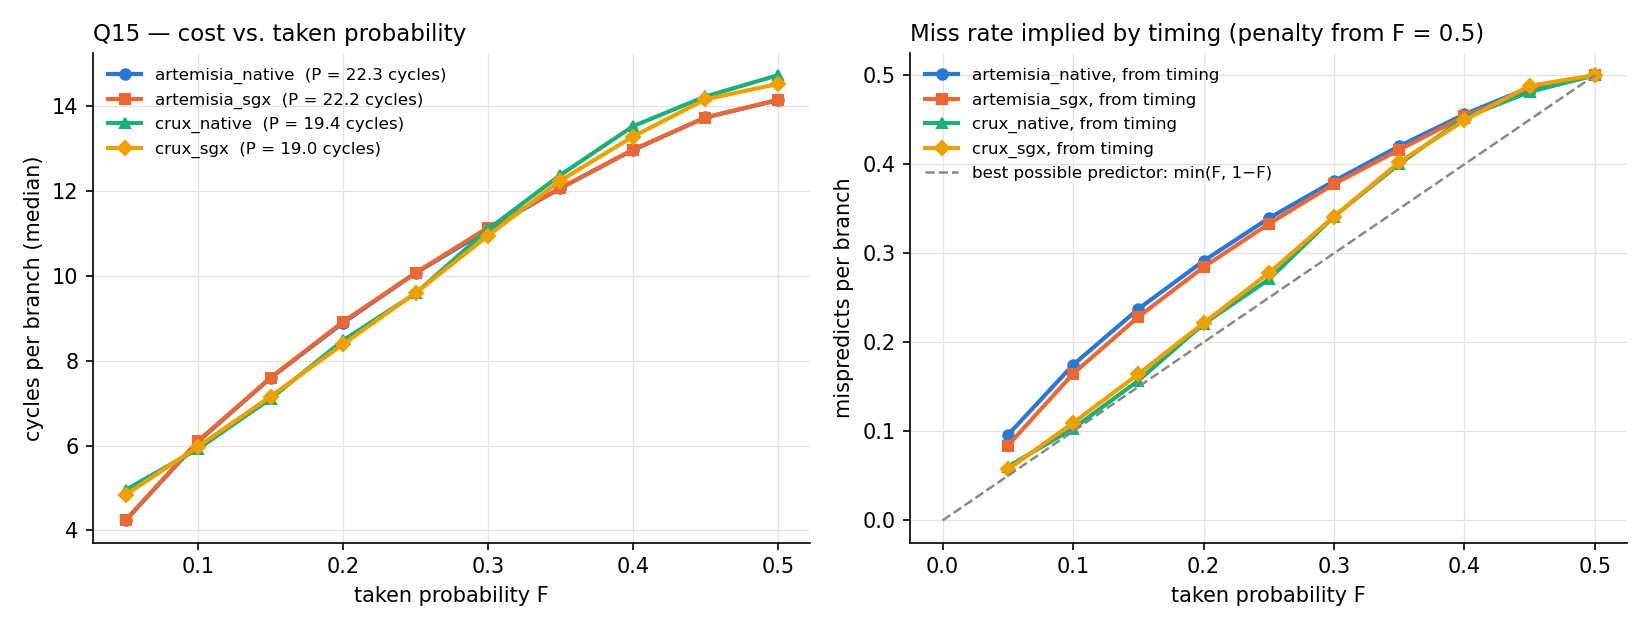
\includegraphics[width=0.95\linewidth]{q15_pipeline_depth/plots/compare/q15_penalty.png}
\caption{Q15, timing only: left, cost against taken probability; right, miss rate implied by timing.}
\end{figure}

\begin{center}
\small
\begin{tabular}{lrrr}
\toprule
Cycles per mispredict & Crux & Artemisia & Artemisia SGX\\
\midrule
\textbf{Timing: fair coin vs.\ \code{alt}} & \textbf{19.4} & \textbf{22.3} & \textbf{22.2}\\
Timing: fair coin vs.\ \code{period:16} & 20.6 & 22.5 & 22.6\\
\midrule
PMU: \code{random} vs.\ \code{alt}, measured miss rate & 18.5 & 23.2 & --\\
PMU: \code{random} vs.\ \code{period:16}, measured miss rate & 19.8 & 22.5 & --\\
PMU: \code{random} vs.\ mean of \code{taken}, \code{nottaken}, measured miss rate & 20.9 & 24.7 & --\\
PMU: slope of cycles against measured miss rate, over \code{bias:F} & 21.6 & 24.0 & --\\
\bottomrule
\end{tabular}
\end{center}

\textbf{Conclusion.} Crux loses about 19--21 cycles per mispredict and Artemisia about 22--23, so Crux has the shorter
refill path. These are lower bounds on fetch-to-execute depth.
\textbf{Enclave:} unchanged (22.2 vs.\ 22.3).
\textbf{PMU check:} the method's assumptions hold, with \code{random} missing at 0.4999 and \code{alt} at about 0 on Crux. PMU
estimates span 18.5--21.6 on Crux and 22.5--24.7 on Artemisia, and timing-implied miss rates are within 0.022 of the PMU on Crux and 0.013
on Artemisia. The remaining uncertainty is the baseline, since no-miss patterns differ in cost. Figure~\ref{fig:q15pmu} shows
the validation. Its per-$F$ values for Crux read low at small $F$ (down to 10.7) because that calculation's baseline rises toward
\code{alt}, which is expensive on Crux; those values should not be taken as the penalty.

\begin{figure}[H]\centering
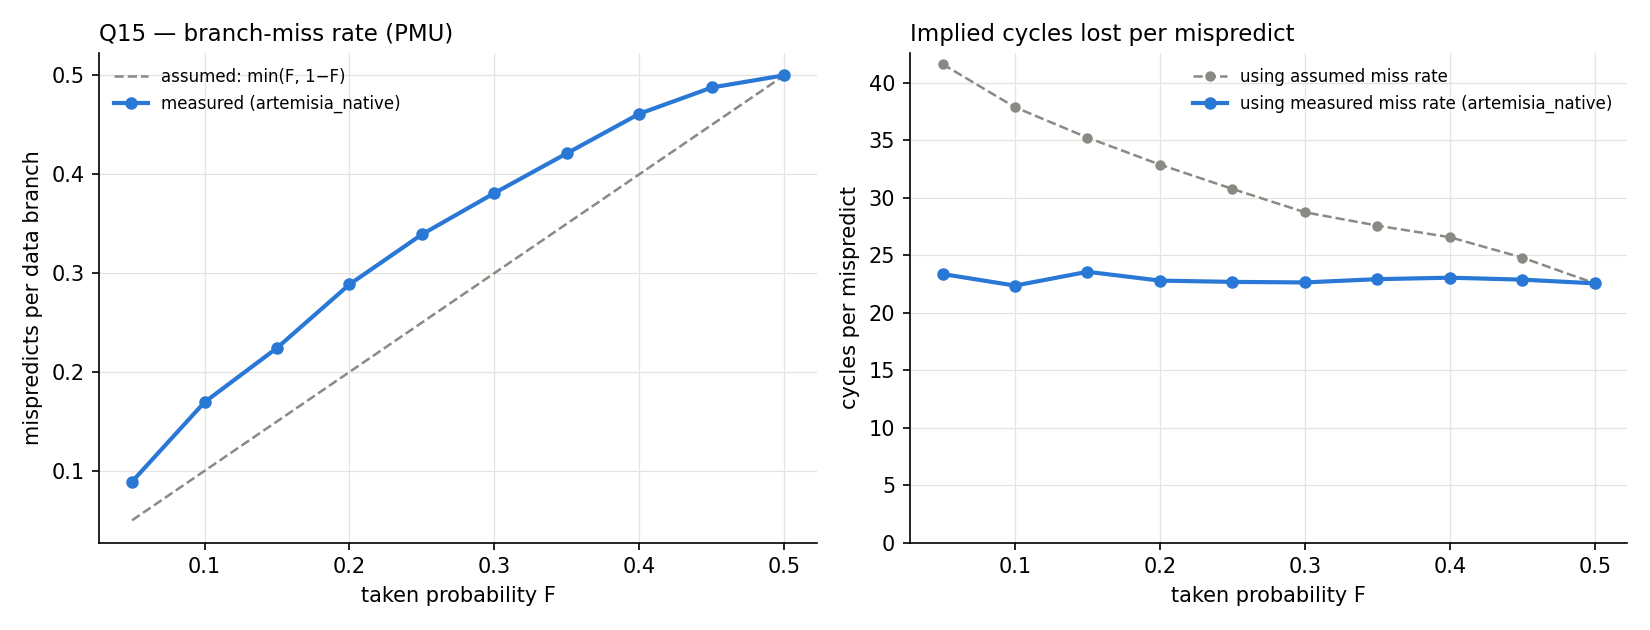
\includegraphics[width=0.95\linewidth]{q15_pipeline_depth/plots/compare/q15_pmu.png}
\caption{Q15, PMU validation only: measured miss rate, and penalty implied by the assumed and measured rates.}
\label{fig:q15pmu}
\end{figure}

\section{Q14: How many instructions are fetched per cycle?}
\textbf{Method.} Long unrolled blocks of NOPs of each length $L$ = 1--15 bytes leave the front end as the only limit. With short NOPs the
limit is instructions per cycle, so IPC flattens. With long NOPs the limit is bytes per cycle, so bytes per cycle flattens and IPC falls
as $1/L$. The block size $K$ selects the path: a small $K$ runs from the micro-op cache, which measures delivery rather than fetch, and a larger $K$ forces legacy fetch and decode.

\begin{lstlisting}
nop_4_4096:
1:  .rept 4096
    .byte 0x0f, 0x1f, 0x40, 0x00     # nopl 0x0(%rax)
    .endr
    dec %rdi
    jnz 1b
    ret
\end{lstlisting}

\begin{figure}[H]\centering
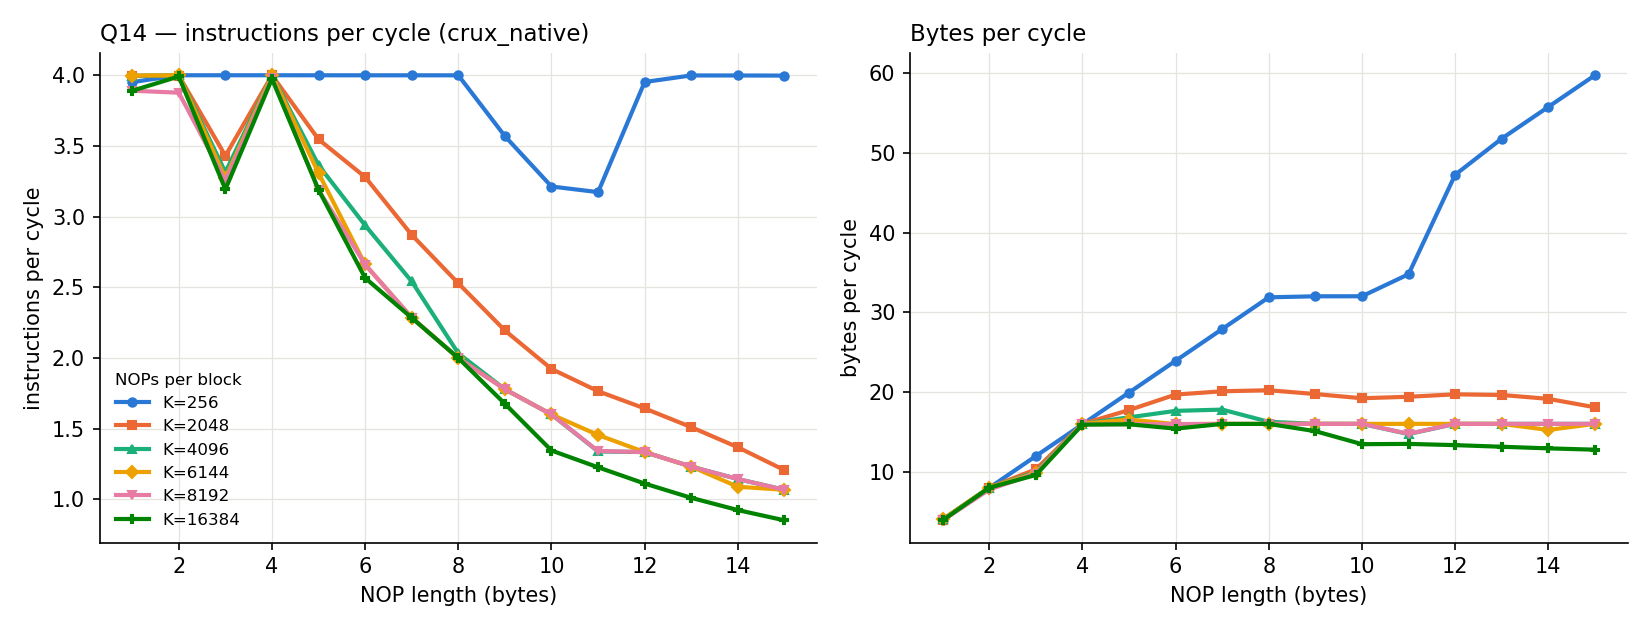
\includegraphics[width=0.88\linewidth]{q14_fetch_width/plots/compare/q14_fetch_crux_native.png}

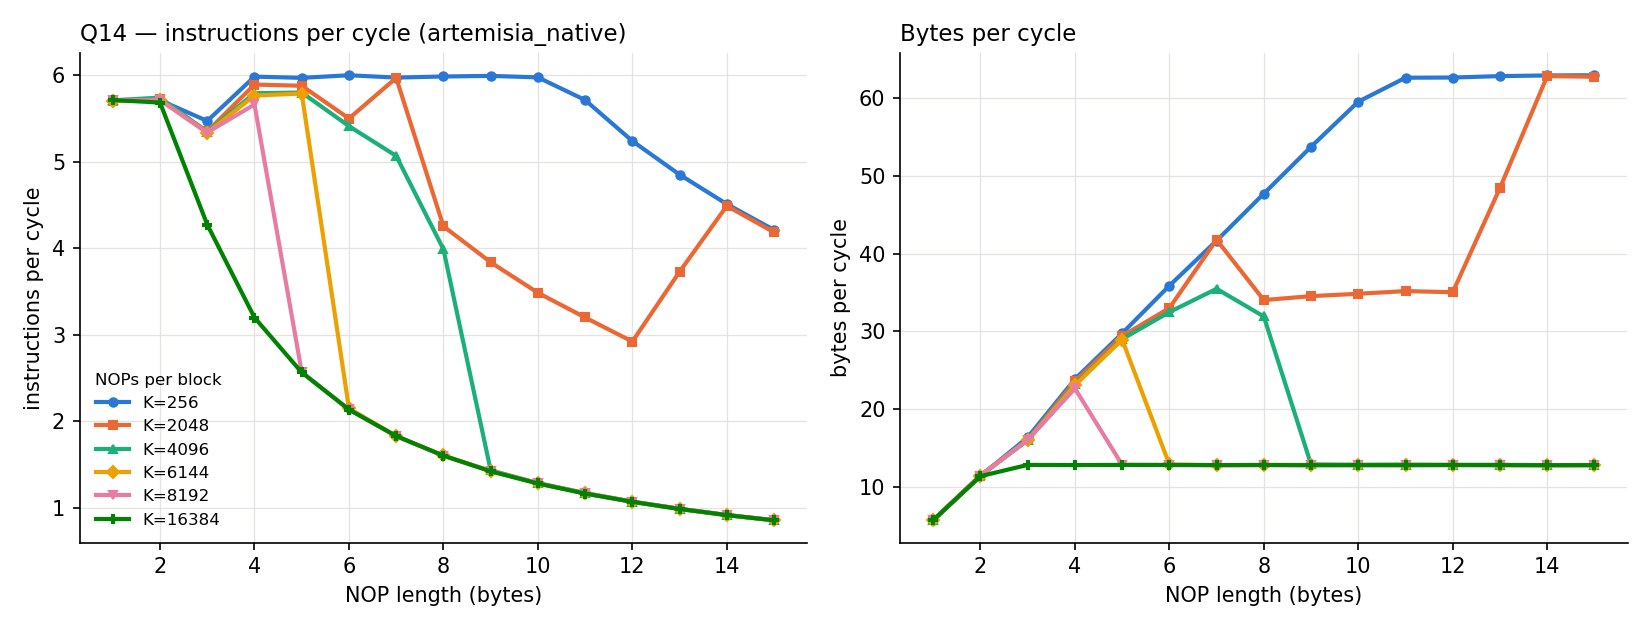
\includegraphics[width=0.88\linewidth]{q14_fetch_width/plots/compare/q14_fetch_artemisia_native.png}
\caption{Q14, native: Crux (top) and Artemisia (bottom). The Artemisia SGX figure is effectively identical and is in the repository.}
\end{figure}

\begin{center}
\small
\begin{tabular}{lll}
\toprule
 & Crux (native) & Artemisia (native and SGX)\\
\midrule
IPC ceiling & 4.0 & about 6.0\\
Legacy fetch ceiling & 16 B/cycle ($K$ = 6144, $L \geq$ 5) & $\geq$29 B/cycle ($K$ = 6144, $L$ = 5)\\
Micro-op cache path ($K$ = 256) & up to about 60 B/cycle & up to about 63 B/cycle\\
Large footprint & about 13 B/cycle ($K$ = 16384, $L \geq$ 10) & 12.8 B/cycle (past 32 KiB)\\
\bottomrule
\end{tabular}
\end{center}

\textbf{Conclusion.} Crux fetches and decodes about 4 instructions per cycle with a clean 16 B/cycle legacy limit. Artemisia sustains about 6 per cycle
with a legacy rate of at least 29 B/cycle; its ceiling was not reached before the footprint passed 32 KiB.
\textbf{Machine difference:} Artemisia falls to 12.8 B/cycle as soon as the footprint passes 32 KiB. Crux instead holds about 16 B/cycle
to roughly 150 KiB before dropping, and I did not determine why.
\textbf{Enclave:} identical to native.
\textbf{PMU check:} whole-program totals only, which cannot confirm the per-path limits, so this is not treated as validation.
\textbf{Open item:} on Crux, 3-byte NOPs reach only about 3.3 IPC with legacy decode, below the neighbouring lengths. This is unexplained.

\section{Q4: How large is the ROB?}
\textbf{Method.} This follows Henry Wong's technique (``Measuring Reorder Buffer Capacity,'' 2013), extending Q2. A missing load A blocks retirement
at the head of the ROB. An independent load B can overlap with it only if B is already allocated, which requires
$N + 2 \le$ ROB size. Below that limit an iteration costs about 1 miss, and above it about 2. NOPs are the filler because
they occupy a ROB entry but write no register and need no scheduler or load/store entry, so the ROB fills first.
I sweep coarsely (step 8), then at step 1 around each machine's own knee.

\begin{lstlisting}
1:  mov (%rax), %rax    # miss A
    nop                 # ... N NOPs
    mov (%rcx), %rcx    # miss B (independent chain)
    nop                 # ... N NOPs
    dec %rdx
    jnz 1b
\end{lstlisting}

\begin{figure}[H]\centering
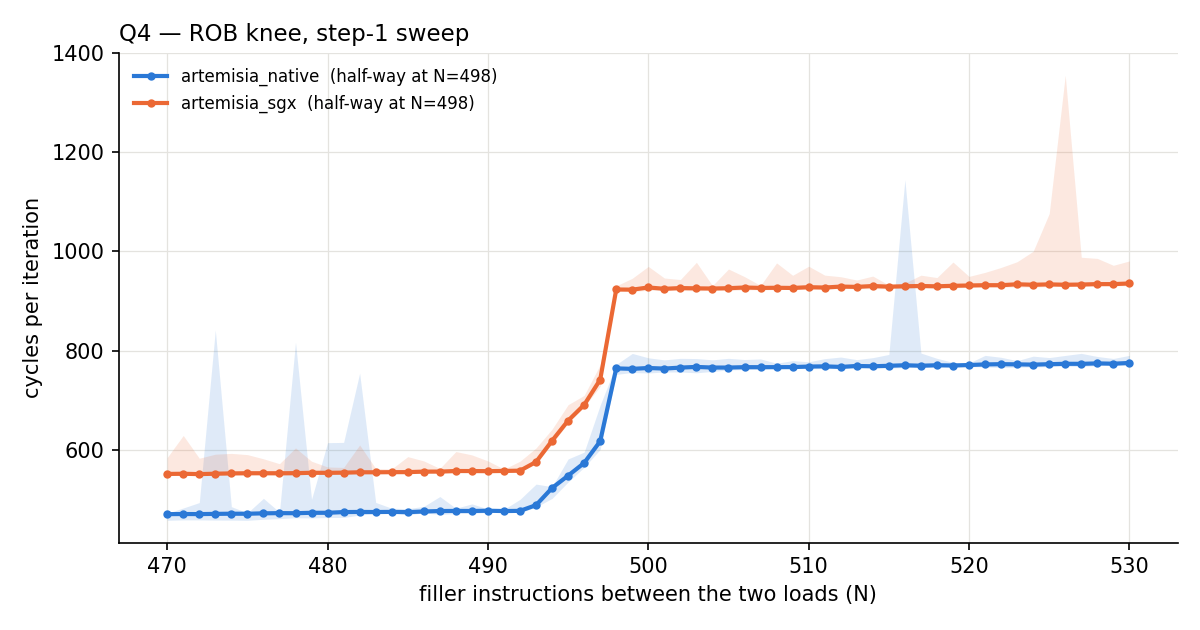
\includegraphics[width=0.72\linewidth]{q04_rob/plots/compare/q4_rob_zoom.png}
\caption{Q4: step-1 sweep around each machine's knee (21 trials).}
\end{figure}

\begin{center}
\small
\begin{tabular}{lrrr}
\toprule
 & Crux native & Artemisia native & Artemisia SGX\\
\midrule
Overlap holds up to & about $N$ = 218 & about $N$ = 492 & about $N$ = 492\\
Partial ramp & 219--222 & 493--497 & 493--497\\
Fully serialized from & \textbf{$N$ = 223} & \textbf{$N$ = 498} & \textbf{$N$ = 498}\\
Per-trial halfway crossing & 223 in 21 of 21 trials & 497--498 in 18 of 21 & 497--498 in 21 of 21\\
Cycles just below / at the knee & 550 / 750 & 617 / 764 & 741 / 923\\
\midrule
\textbf{Measured ROB} & \textbf{224--225} & \textbf{499--500} & \textbf{499--500}\\
Published (not measured) & 224 & 512 & 512\\
\bottomrule
\end{tabular}
\end{center}

\textbf{Conclusion.} ROB is about 224--225 entries on Crux and about 499--500 on Artemisia. The range reflects whether the first
serialized $N$ is read as ROB $-$ 1 or ROB $-$ 2.
\textbf{Machine difference:} Crux matches its published size, while Artemisia measures about 12 entries (2.3\%) below its published size. I can't
explain this gap from the data, nor the short ramp before each knee.
One untested hypothesis is that the previous iteration's load B can still be at the ROB head when load A issues.
\textbf{Enclave:} the knee does not move, and only the plateaus rise, because enclave misses cost more.
\textbf{PMU check:} not performed.

\section{Q5: How large is the physical register file, and of which class?}
\textbf{Method.} This uses the Q4 loop, but every filler instruction writes a register, and that write holds a physical register until retirement.
If registers run out before the ROB does, the knee moves to a smaller $N$, giving the number of \emph{free} registers of that class.
\code{int} uses \code{add r,r} and \code{ymm} uses \code{vpaddd}. Zeroing idioms and \code{mov r,r} are avoided, because rename can handle them without allocating a register.
\code{mix} alternates the two: with one shared file, the knee would stay near the smaller single-class knee; with separate files, each
fills at half the rate, so the knee moves out until twice the integer knee or the ROB limits it. Controls vary flag-writing, chains and immediates.

\begin{lstlisting}
1:  mov (%rax), %rax    # miss A
    add %r8, %r8        # int filler: each writes a fresh physical register
    add %r9, %r9
    vpaddd %ymm0, %ymm0, %ymm1   # ymm filler; mix alternates add and vpaddd
    mov (%rcx), %rcx    # miss B
    ...
\end{lstlisting}

\begin{figure}[H]\centering
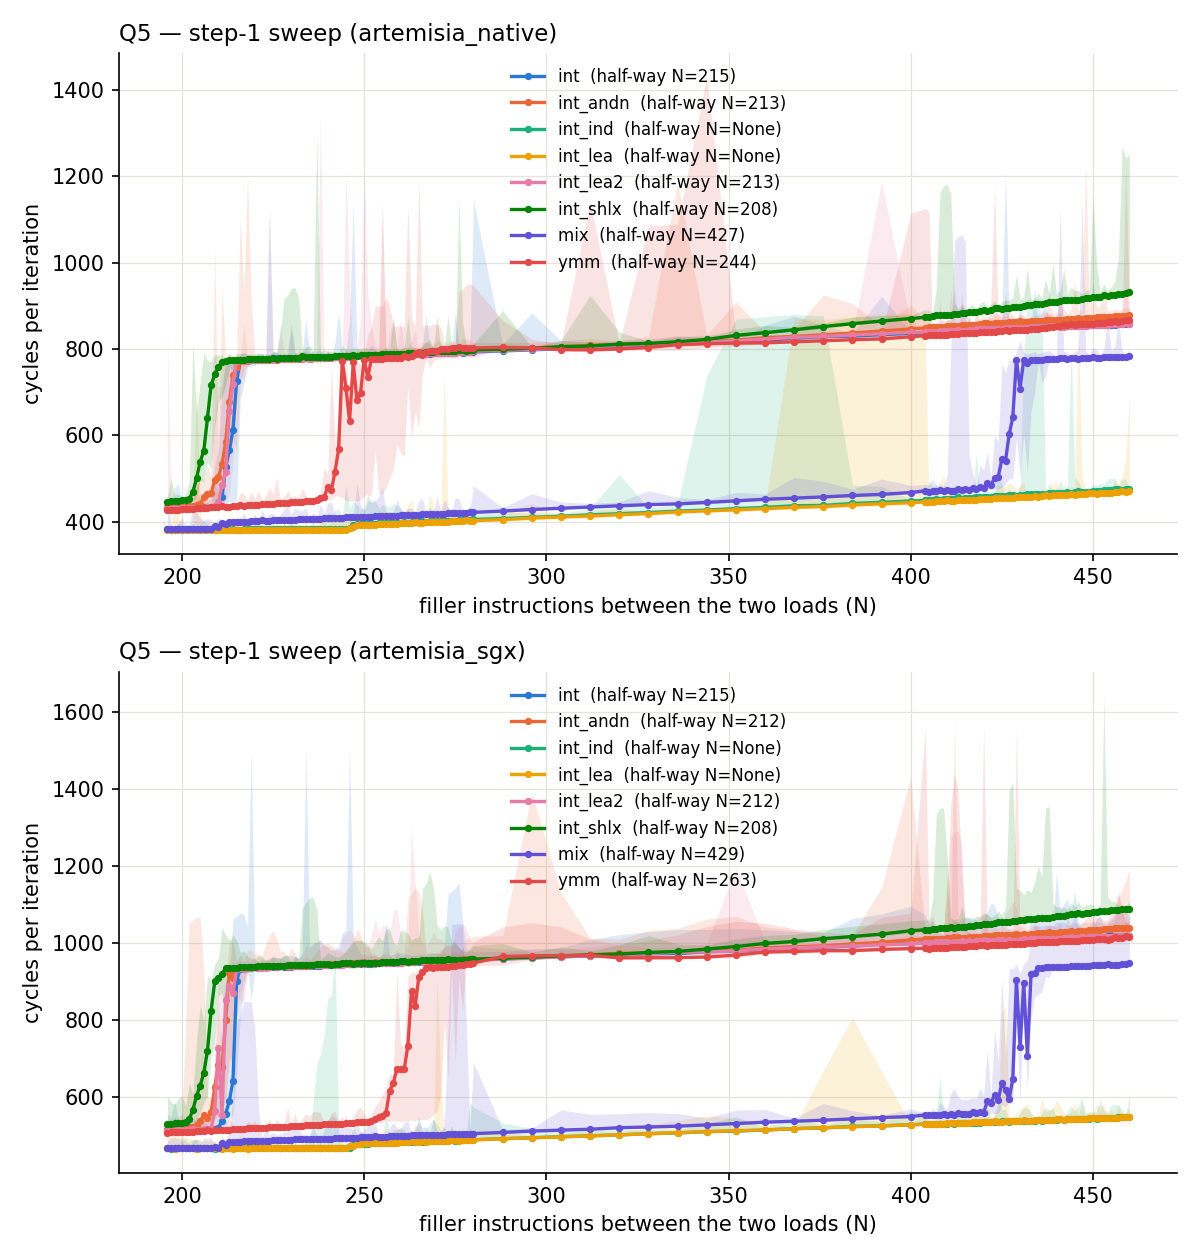
\includegraphics[height=0.62\textheight]{q05_prf/plots/compare/q5_prf_zoom.png}
\caption{Q5: step-1 sweeps (21 trials). Labels give the halfway crossing for each filler.}
\end{figure}

\begin{center}
\small
\begin{tabular}{llrrr}
\toprule
Filler & Writes & Crux native & Artemisia native & Artemisia SGX\\
\midrule
\code{nop} (Q4) & Nothing & 223 & 498 & 498\\
\code{add r,r} (\code{int}) & GPR + flags & \textbf{145} & \textbf{215} & \textbf{215}\\
\code{andn} & GPR + flags & 143 & 213 & 212\\
\code{shlx} & GPR only & 143 & 208 & 208\\
\code{lea (r,r)} & GPR only & 138 & 213 & 212\\
\code{lea 1(r)} & GPR only, reg+imm & 142 & No PRF knee & No PRF knee\\
\code{lea 1(rbp)} & GPR only, reg+imm & 142 & No PRF knee & No PRF knee\\
\code{vpaddd ymm} & Vector & \textbf{148} & \textbf{244} & \textbf{263}\\
\code{mix} & Both, alternating & \textbf{208} & \textbf{427} & \textbf{429}\\
\midrule
\multicolumn{2}{l}{Published integer PRF (not measured)} & 180 & 280 (see below) & \\
\multicolumn{2}{l}{Published vector PRF (not measured)} & 168 (see below) & about 332 & \\
\bottomrule
\end{tabular}
\end{center}

\textbf{Conclusions.}
\begin{itemize}
\item \textbf{Register sizes:} about 145 free integer and 148 free vector registers on Crux, and about 215 and 244 on Artemisia. These
are free counts, so the total is a lower bound: committed architectural state, at least 16 GPRs, occupies entries too.
\item \textbf{Register class:} integer and vector are separate files on both machines, since \code{mix} runs well past both single-class knees. On Artemisia it reaches
about twice the integer knee. On Crux twice the integer knee (290) exceeds the ROB, so the ROB should cap it.
\item \textbf{Flags:} not a separate limit, since flag-writing and flag-free fillers give the same knee.
\item \textbf{Machine difference:} on Artemisia, \code{lea} with a register plus immediate shows no register limit and runs to the ROB, which suggests
rename handles it without allocating a register. On Crux the same instruction hits the normal limit.
\end{itemize}

\textbf{Enclave.} Integer and \code{mix} knees are unchanged. The vector knee is 263 in the enclave against 244 natively. This appears to be architectural state rather than a hardware effect: writing \code{ymm16--31} first moves the enclave's median knee to 244 and changes nothing natively. In-use bits
from \code{xgetbv(1)} show that glibc leaves those registers in use in a native process, and the enclave's libc does not.
The matching native sweep with glibc's AVX-512 paths disabled gave 255 in one noisy run, so that step is unconfirmed.

\textbf{Open questions.} On Crux, \code{mix} at 208 is about 15 short of the ROB knee (223), and I have no explanation. The separate-files conclusion
does not depend on it. The knees also sit below published totals by more than 16 architectural registers (Crux: 145 + 16 = 161 vs.\ 180; Artemisia: 215 + 16 = 231 vs.\ 280, where an idle SMT
sibling's state could account for part of the gap). The published Skylake vector count of 168 and Golden Cove integer count of 280 come from secondary sources that I could not
confirm against a primary one, and the Golden Cove vector count was measured by Chips and Cheese as about 327.
\textbf{PMU check:} not performed; the stall-event names vary by generation.

\section{Challenges and limitations}
\begin{itemize}
\item \textbf{SGX on Artemisia and tooling.} SGX was first disabled in BIOS, and then access needed the \code{sgx} group. Gramine's install was incomplete, so
the enclave backend was built on the Intel SGX SDK instead, after confirming \code{rdtsc} works natively inside the enclave with the same resolution (calibration within 0.6\%).
\item \textbf{SGX on Crux.} No access: SGX is off in firmware, so Crux is native only.
\item \textbf{No-SMT crash.} The first Crux run produced no data: with no sibling, the harness's sibling lookup matched nothing, and \code{set -e} with \code{pipefail} ended each script before the benchmark ran. This was fixed in the shared harness and doesn't affect Artemisia's results.
\item \textbf{Clock changes on Crux.} The calibrated clock usually measured about 4.68 GHz but fell as low as about 4.48 GHz, consistent with turbo limits as other cores wake (not confirmed). In the first run this distorted Q1 and Q2 (\code{add\_dep} read 0.957), so both were rerun. The final Q1 and Q2 data show drift of at most 0.02\%. Occasional dips remain in the min--max bands.
\item \textbf{Biased-coin analysis.} The first Q15 analysis treated min($F$, $1-F$) as the miss rate, so the ``penalty'' drifted from 43 to 22 cycles. These values are upper bounds, and the method now uses only the fair coin.
\item \textbf{Bimodal timing.} On Artemisia, \code{taken} and \code{nottaken} flip between about 2.0 and 3.2 cycles from trial to trial, for an unknown reason. It affects small-$F$ estimates but not the Q15 result. Other users' load also caused whole-trial slowdowns, visible in the bands but not the medians.
\item \textbf{Questions not attempted.} TLB (6--9), BTB (10--12), predictor type (13) and SMT sharing (16) were not selected.
\end{itemize}

\section{AI use}\label{sec:ai}
Track B, with AI use disclosed. Claude Chat (Anthropic) helped me with the original plan, including the question selection. I then used Claude Code (Anthropic) in the VS Code extension, with Claude Opus 5.5 for the logged sessions. It wrote most of the harness, ran the experiments and PMU checks on both machines
from my sessions, helped analyse results, and drafted this report. I made the final choice of questions and plan, and the decisions recorded in
\code{AI\_LOG.md}, which is the full log and is included in the submission.

\section{Reproduction}
Requirements: \code{gcc}, \code{make}, \code{python3} with \code{numpy} and \code{matplotlib}. For enclave runs: the Intel SGX SDK in \code{/opt/intel/sgxsdk}, \code{openssl} and a session in the \code{sgx} group.
\begin{lstlisting}
common/preflight.sh 2        # check tools, CPU features, the pin CPU, LLC, SGX, perf
common/run_all.sh 2          # all experiments and zooms, then plots; adds SGX if usable
common/pmu_verify.sh 2       # validation only: needs perf_event_paranoid <= 2
common/plot_all.sh           # figures -> q*/plots/compare/ (all machines overlaid)
common/plot_all.sh crux      # figures -> q*/plots/crux/
\end{lstlisting}
Timing results are in \code{q*/results/<machine>/<mode>.csv}, with step-1 sweeps under \code{zoom/}. PMU results are separate, under \code{pmu/}, and the
validation tables are generated in \code{report/pmu\_tables.md}. Each question's folder has a README with its commands, and \code{machines/} records each machine's \code{lscpu} and \code{cpuinfo}.

\end{document}
